\section{Data}
    % Suggested 300 words

    \paragraph{Data provenance}
        We utilized two movie datasets: an IMDb dataset\cite{data:IMDb} and
            TMD\cite{data:TMD} (The Movie Dataset).
        The IMDb dataset contains data about movies made from 2006-2016, while the TMD
            dataset contains data about movies released on or before July 2017.
        Both datasets were obtained from kaggle.com and are shared under the CC0 1.0
            Universal Public Domain Dedication.
        TMD is merged data from TMDb (The Movie DataBase) and grouplens.org, a movie
            ranking site.
        However, we only used the part that was obtained from TMDb.
        It is worth noting that the provenance of the IMDb dataset has been subject to
            controversy as it was scraped from IMDb.com. 
        However, for this investigation, we used only a sample of this dataset which is publicly
            available on Kaggle.com.

    \paragraph{Data description}
        The IMDb movie dataset contains 12 columns with string or floating point
            values. 
        The only column of note is the Genre column, which can only take on 12 distinct values, 
            shown in Table \ref*{tab-IMDb-Movie-Data-Column-Description}.
        A summary of the columns is provided in Table \ref*{tab-IMDb-Movie-Data-Column-Description}.
        \begin{table}[h]
            \centering
            \begin{tabular}{lp{10cm}l}
                \toprule
                Column Name        & Description                                                                & Data Type \\
                \midrule
                Rank               & The rank the movie has in the IMDb database                                & Integer   \\
                Title              & The name of the movie                                                      & String    \\
                Genre              & The genres that apply to the movie, there can be anywhere from 1-3 genres.
                A genre can be any from: Action, Adventure, Sci-Fi, Thriller, Animation,
                    Comedy, Family, Fantasy, Drama, Music, Romance, History, Crime, Western, War,
                    Musical, Sport, Horror, Mystery, Biography.
                                   & Genre                                                                                  \\
                Description        & The description of the movie                                               & String    \\
                Director           & The person who directed the movie                                          & String    \\
                Actors             & The lead roles in the movie                                                & String    \\
                Year               & The year the movie was released                                            & Integer   \\
                Runtime (Minutes)  & The runtime in minutes of the movie                                        & Integer   \\
                Rating             & The mean rating of the movie, taken from IMDb.com                          & Float     \\
                Votes              & The amount of users that voted on a movie to give it that rating           & Integer   \\
                Revenue (Millions) & The gross income the movie made at the US box office                       & Float     \\
                Metascore          & The rating of movie, determined using aggregated weighted Critics scores   & Integer   \\
                \bottomrule
            \end{tabular}
            \caption[short]{The different columns in the IMDb-Movie-Data.csv file}\label{tab-IMDb-Movie-Data-Column-Description}
        \end{table}

        We worked exclusively with the Crew table in TMD, which is a small part of
            the entire database. 
        This table contains three columns - Cast, Crew, and ID.
        However, the Cast and Crew columns are not composed of discrete data points, 
            but rather JSON files representing the entire cast or crew list. 
        As a result, we to extracted the data using string parsing methods. 
        A summary of the columns is provided in Table \ref*{tab-Credits-Column-Description}.
        \begin{table}[h]
            \centering
            \begin{tabular}{lp{10cm}l}
                \toprule
                Column Name & Description                                                              & Data Type  \\
                \midrule
                cast        & The cast list of the movie, including all actors who appeared in it.     & .json file \\
                crew        & The entire crew list of the movie, including all the people who made it. & .json file \\
                id          & The movie id - used in the larger dataset to connect tables together     & Integer    \\
                \bottomrule
            \end{tabular}
            \caption[short]{The different columns in the credits.csv file}\label{tab-Credits-Column-Description}
        \end{table}

    \paragraph{Data processing}
        We used a Python script to parse the TMD dataset and count the number of
            movies each director and actor has been involved in.
        The resulting datasets were saved as CSV files named actor\_counts.csv and
            director\_counts.csv.
        We then merged this data with the original IMDb
            dataset.
        This involved dropping the Description column and replacing the
            Director and Actor columns with Director Exp. and Mean Lead Roles Exp.
        A summary of the merged datasets columns is shown in Table
            \ref*{tab-merged-data-column-description}.

        \begin{table}[h]
            \begin{tabular}{lp{9cm}l}
                \toprule
                Column Name          & Description                                                  & Data Type \\
                \midrule
                Rank                 & See table \ref{tab-IMDb-Movie-Data-Column-Description}       & Integer   \\
                Title                & See table \ref{tab-IMDb-Movie-Data-Column-Description}       & String    \\
                Genre                & See table \ref{tab-IMDb-Movie-Data-Column-Description}       & Genre     \\
                Director Exp.        & The number of movies that the director of the movie has made & Float     \\
                Mean Lead Roles Exp. & The mean number of movies that the lead actors have been in  & Float     \\
                Year                 & See table \ref{tab-IMDb-Movie-Data-Column-Description}       & Integer   \\
                Runtime (Minutes)    & See table \ref{tab-IMDb-Movie-Data-Column-Description}       & Integer   \\
                Rating               & See table \ref{tab-IMDb-Movie-Data-Column-Description}       & Float     \\
                Votes                & See table \ref{tab-IMDb-Movie-Data-Column-Description}       & Integer   \\
                Revenue (Millions)   & See table \ref{tab-IMDb-Movie-Data-Column-Description}       & Float     \\
                Metascore            & See table \ref{tab-IMDb-Movie-Data-Column-Description}       & Integer   \\
                \bottomrule
            \end{tabular}
            \caption[short]{The different columns in the merged data set}\label{tab-merged-data-column-description}
        \end{table}

        To check this data was properly normalised we made a histogram plot of all the
            numeric variables, shown in Figure \ref{fig-distribution-of-numeric-variable}.
        As expected, a few variables did not appear to be normally distributed, namely:
        Revenue (Millions), Votes, Runtime (Minutes), Director Exp., and Rating.
        \begin{figure}[H]
            \centering
            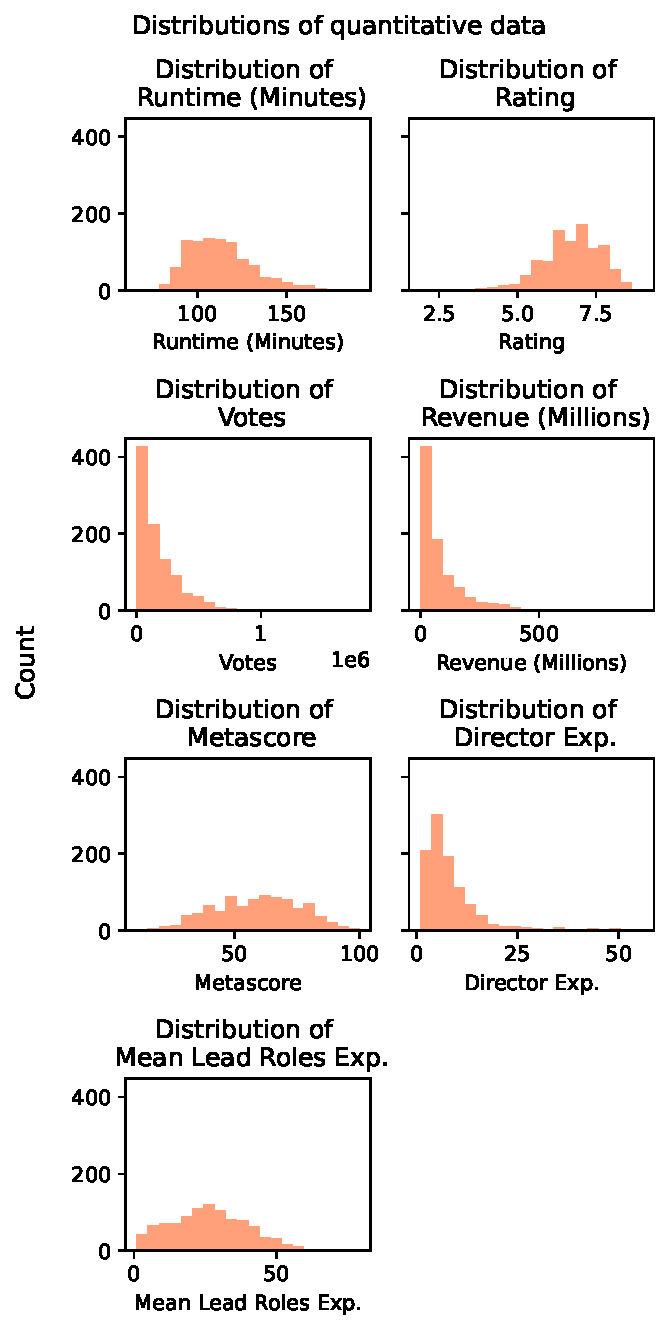
\includegraphics[width=0.8\linewidth]{Final/Distribution of Numeric Variables (No Transformation).pdf}
            \caption[short]{The distributions of the numeric variables in the merged dataset}\label{fig-distribution-of-numeric-variable}
        \end{figure}
        Figure \ref*{fig-distribution-of-numeric-variable} shows that Revenue (Millions) and Votes are
        severely right-skewed, implying an exponential distribution. Runtime
        (Minutes) and Director Exp. appear to be less severely right-skewed,
        implying a lognormal distribution. Rating seems to be left-skewed. The
        transformations that give the best approximations to a normal
        distribution are cube root transform for Revenue (Millions) and Votes,
        log transform for Runtime (Minutes) and Director Exp., and square
        transform for Rating.
        \begin{figure}[H]
            \centering
            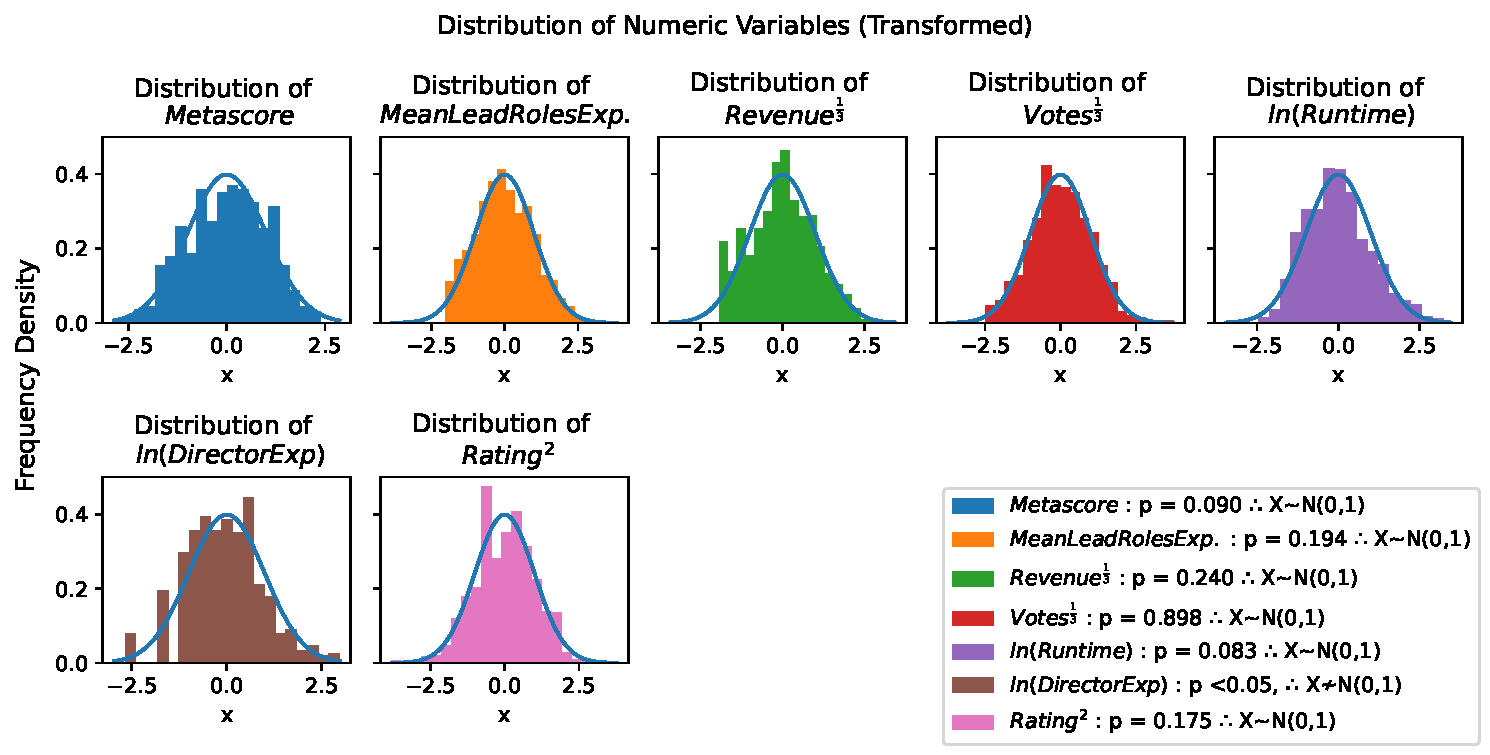
\includegraphics[width=\linewidth]{Final/Distribution of Numeric Variables (Transformed).pdf}
            \caption[short]{The distributions of the standardised and normalised numeric variables in the merged dataset,
                            the legend has the p-values from testing with $H_{0}: X \not\sim N(0,1)$. Also shown on the plots is
                            the Gaussian Distribution with the columns mean and standard deviation}\label{fig-transformed-distribution-of-numeric-variable}
        \end{figure}
        Figure \ref*{fig-transformed-distribution-of-numeric-variable} shows the
        standarised and normalised numeric variables. The legend contains the p-values
        from the Kolmogorov-Smirnov normality test \cite*{KStest}, which was used to
        test the data against the null hypothesis $H_{0}: X \not\sim N(0,1)$. It is
        worth noting that the Director Exp. column failed the test, however, there is
        missing data present in the histogram. Despite this, the histogram follows a
        normal distribution curve, providing convincing evidence that ln(Director Exp.)
        has a normal distribution. Ultimately, these transformations helped to normalize
        the dataset and improve its suitability for further analysis.

        To make use of the Genre column, one-hot encoding was used.
        We added a column for each Genre and set each entry to 1 if the corresponding movie
            fit that genre and 0 otherwise.
        Genres with less than 100 movies made were excluded to ensure a large enough sample size
            was present, such that we could draw meaningful conclusions